\chapter{Обзор предметной области}\label{ch:ch1}

\section{Антагонистические игры и случайные блуждания}\label{sec:ch1/sec1}

Теория игр тесно переплетается с проблемами случайных блужданий в широком спектре областей прикладных и фундаментальных исследований 
от хемотаксиса бактерий и рыночных взаимодействий до блужданий роя автономных роботов и компьютерных игр \cite{}. 
Игры, в которых возникают случай влияет на развитие игровой ситуации, могут быть рассмотрены как случайное блуждание
на некотором графе всех возможных конфигураций предметов игры или в некотором непрерывном пространстве всех возможных состояний.
В общем случае окончание таких игр определяется при возникновении некоторой предопределенной выигрышной траектории.
Одной из таких возможных ситуаций является поглощение траектории в некотором состоянии при случайном блуждании в пространстве конфигураций.
В зависимости от типа игры игрокам может требоваться оптимизировать длительность случайного блуждания или расставить поглощающие состояния 
так, чтобы раньше другого игрока поймать траекторию \cite{}. Одной из самых простых игр такого типа является задача о разорении игрока \cite{}
и различные её модификации \cite{}. Обобщение случайных блужданий игрового типа было проведено в работе И.~В.~Романовского \cite{romanovskiy_1961}.
Рассматриваемые теорией игр процессы обусловлены взаимодействием одного игрока с некоторой системой, двух игроков или множества игроков.
В последующих разделах проведен анализ первых двух случаев, соответствующих антагонистическим играм между двумя игроками с противоположными интересами.

\subsection{Задача о разорении игрока}\label{subsec:ch1/sec1/sub1}

Впервые упоминание о задаче разорения игрока появилось в переписке Блеза Паскаля и Пьера Ферма в 1656 году при рассмотрении игры тремя костями между двумя игроками.
Первый игрок получал очки при выпадении суммы на игральных костях равной 11, а второй игрок при выпадении суммы равной 14. Однако, способ начисления очков 
был модифицирован: очко добавляется к счету игрока только в том случае, если счет его противника равен нулю, а в противном случае очко будет вычтено из счета его противника.
В этом случае счет отстающего игрока всегда остается равным нулю. Первый из игроков набравший 12 очков объявлялся победителем. В переформулированной версии
письма Пьером де Каркави, направленной Христиану Гюйгенсу в 1656 году, вопрос к задаче состоял в нахождении вероятности победы первого и второго игрока. 

В своей работе De ratiociniis in ludo aleae Христиан Гюйгенс получил более приближенную формулировку к классической: игроки начинают с 12 очков, успешный бросок 
трех костей (11 для первого и 14 для второго) добавляет этому игроку одно очко и вычитает у второго, при этом первый достигший нуля очков проигрывает.
Вопрос как и ранее состоял в нахождении вероятности победы игроков. 

Классическая формулировка обобщает для одномерного случая задачу о разорении игрока для случая произвольных начальных условий и произвольных вероятностей перехода. 
Пусть у первого игрока есть $-A$ монет ($A < 0, -A > 0$), у второго игрока - $B$ монет. На каждом ходу подбрасывается ассиметричная монета, имеющая вероятность выпадения 
аверса $p$ и реверса $1-p$. При выпадении аверса одна монета переходит от второго игрока к первому, при выпадении реверса - наоборот. Требуется найти вероятность проигрыша 
за $n$ шагов, а также общую вероятность проигрыша каждого из игроков. В дополнение к формулировке Христиана Гюйгенса ставится вопрос о среднем времени игры, 
где время игры характеризует количество ходов до проигрыша одного из игроков.

Тесная связь со случайными блужданиями позволяет сформулировать данный процесс в виде дискретного блуждания частицы по целочисленному отрезку $[A; B]$, 
при этом выход на границу отрезка характеризует проигрыш одного из игроков. 

Решение задачи состоит в рассмотрении схемы Бернулли с последовательностью Бернуллиевских случайных величин $\xi_i$ с вероятностью $p$ дающих $+1$ и 
с вероятностью $q=1-p$ значение $-1$.
Тогда сумма таких величин $S_k=\sum_{i=1}^{k} \xi_i$ равна случайной величине, соответствующей положению частицы в случайном блуждании на отрезке $[A; B]$.
Вводя обозначения для вероятностей завершить игру в точках $A$ и $B$ за время $[0; k]$ при старте в позиции $x$ соответственно $\alpha_k(x), \beta_k(x)$ 
запишем рекуррентные соотношения:

\begin{equation}
    \label{eq:eq1}
    \begin{alignedat}{2}
        \alpha_k(x) = p\alpha_{k-1}(x+1)+q\alpha_{k-1}(x-1),\\
        \beta_k(x) = p\beta_{k-1}(x+1)+q\beta_{k-1}(x-1).
    \end{alignedat}
\end{equation}

При достаточно больших $n$ решение рекуррентного соотношения близко к стационарной точке точечного отображения при заданных граничных условиях:
\begin{equation}
    \label{eq:eq2}
    \begin{alignedat}{2}
        \alpha(x) = p\alpha(x+1)+q\alpha(x-1), \alpha(A)=1, \alpha(B)=0,\\
        \beta(x) = p\beta(x+1)+q\beta(x-1), \beta(A)=0, \beta(B)=1.
    \end{alignedat}
\end{equation}

Поиск решения уравнения в форме $(q/p)^{x}$ дает следующий результат:
\begin{equation}
    \label{eq:eq2}
    \begin{alignedat}{2}
        \alpha(x) = ((q/p)^B-(q/p)^x)/((q/p)^B-(q/p)^A),\\
        \beta(x) = ((q/p)^x-(q/p)^A)/((q/p)^B-(q/p)^A).
    \end{alignedat}
\end{equation}

При справедливой игре $(p=q)$ выражения для определения вероятностей редуцируются до линейной формы:
\begin{equation}
    \label{eq:eq2}
    \begin{alignedat}{2}
        \alpha(x) = (B-x)/(B-A),\\
        \beta(x) = (x-A)/(B-A),
    \end{alignedat}
\end{equation}
где $x \in [A; B]$ --- стартовое положение на отрезке.

Заключительный аспект задачи о разорении игрока состоит в исследовании среднего времени достижения финального состояния.
С точки зрения случайных блужданий процесс представляется в виде Марковской цепи с поглощающими состояниями на концах отрезка 
и промежуточными состояниями в целочисленных координатах отрезка. Рассмотрим подход к решению задачи о нахождении математического
ожидания времени окончания игры $m_k(x)$ для некоторой игры длины $k$ находящейся в состоянии $x$. Тогда рекуррентное соотношение 
для соседних состояний представляется в виде:
\begin{equation}
    \label{eq:eq2}
    m_k(x) = p m_{k-1}(x + 1) + q m_{k-1}(x - 1) + 1, x \in (A, B), k > 0,
\end{equation}

На границе в точках $A$, $B$ количество ходов для завершения игры равно нулю, то есть $m_k(A) = m_k(B) = 0$.
С учетом конечности математического ожидания пределом при $k->\infty$ будет являться решение рекуррентного соотношения 
$m(x)=p m(x+1) +q m(x - 1) + 1$. Итоговое решение для общего случая представляется в виде:

\begin{equation}
    \label{eq:eq2}
    m(x) = 1 / (p - q) (B \beta(x) + A \alpha(x) - x)
\end{equation}

При симметричной монетке формула упрощается до $m(x) = (B - x) (x - A)$, а в случае равного начального капитала $m(x) = B^2$.

Таким образом оценки позволяют найти как вероятность выигрыша каждого из игроков в зависимости от параметров игры, так и среднее время игры.

\subsection{Задача о разорении игрока с несколькими валютами}\label{subsec:ch1/sec1/sub2}

Обобщение задачи о разорении игрока на двумерный случай было рассмотрено израильскими математиками в 1994 году \cite{}. 
Для решения задачи был применен метод производящих функций и получены выражения для случая с равновероятными переходами на отрезке и на квадратной решетке.
Применяя символьные вычисления в пакете MAPLE \cite{} тем же способом было найдено решение с произвольными вероятностями перехода в 4 направлениях 
на четырех-связной решетке. 

Естественным продолжением двумерного случая является обобщение на произвольные размерности. В 2000 году Марко Петковсек и Андреем Кмет 
рассмотрели задачу о разорении игрока, в которой имеется несколько различных валют. \cite{}
Формулировка игровой механики для многомерного случая состоит в равновероятном выборе валюты и победителя на каждом ходу.
В результате хода победитель забирает одну монету выпавшей валюты у проигравшего. Игра продолжается до тех пор, пока у одного из игроков не закончатся монеты любой из валют.
В своей работе словенские математики получили среднее время игры в явной форме для случая равновероятных переходов между соседними узлами решетки
с применением дискретного преобразования Фурье и выражений для спектра симметричной тридиагональной матрицы Теплица.
Полученное выражение для среднего времени игры в зависимости от начального капитала игроков состоит из двойной суммы для двумерного случая 
и может быть вычислено за время $O(N^2)$: 
\begin{equation}
    \label{eq:eq2}
    a_{ij} = 4 / N^2 \sum_{k=1\\ k odd}^{N - 1} sin(jk\pi/N)cot(k\pi/(2N)) \sum_{l=1\\ l odd}^{N - 1} sin(il\pi/N)cot(l\pi/(2N))/(sin^2(k\pi/(2N))+sin^2(l\pi/(2N))),
    0 <= i, j <= N
\end{equation}
Хотя авторы не получили более быстрый алгоритм для общего случая, высказано предположение о возможности получения выражения в виде одной суммы.
Явные формулы в виде одной суммы (вычислительная сложность $O(N)$) были получены для частного случая стартовых капиталов одинакового размера являющегося степенью 2.
Также математики получили решение для многомерного случая на базе уравнения Сильвестра и тензорного спектрального разложения.

\subsection{Случайные блуждания}\label{subsec:ch1/sec1/sub3}

Первое появление термина "случайные блуждания" относится к письму Карла Пирсона в редакцию журнала Nature в 1905 году \cite{}.
Мотивированный проблемами, возникшими в биологии, он сформулировал следующую задачу:
"Человек начинает путешествие из точки O и проходит l ярдов по прямой линии. 
Затем он поворачивается на какой угодно угол, и проходит еще l ярдов по прямой линии. 
Он повторяет этот процесс n раз. Я ищу вероятность того, что после этих n прогулок он окажется 
на расстоянии между r и r+dr от своей начальной точки O."

На письмо ответил британский физик Лорд Рэлей, который ранее в своей работы 1880 года от теории звука рассмотрел
n изопериодических колебаний единичной амплитуды и фазы, распределенные случайным образом. Для достаточно больших n 
Рэлей нашёл асимптотическое решение в замкнутой форме, отражающее распределение вероятностей в задаче Карла Пирсона. 

Решение задачи для многомерного случая в евклидовом пространстве представляется существенно более сложной задачей в связи с чем в своих работах Лорд Рэлей
рассматривал модель случайного блуждания на решетке. Исследуя случайные блуждания на решетке Дьёрдь Пойа в своих работах 1919 и 1921 года \cite{} показал, что, 
в случае случайного блуждания на решетке с равновероятными переходами во всех направлениях в одномерном и двумерном случаях, 
агент возвращается в исходную точку с вероятностью 1, а для размерностей больше двух с вероятностью 0.

Как заметил профессор прикладной математики Невилл Темперлей, различные комбинаторные задачи, возникающие при изучении 
разнообразных физических явлений, связанных с решетками, могут быть разрешимы в терминах подсчета числа траекторий случайного блуждания с ограничениями \cite{}. 
Задачи, возникающие в различных областях таких как химия, физика, экономика, биология, сводились к анализу случайных блужданий на решетках со сложной структурой и 
особыми ограничениями \cite{, , , ...}. 

После публикации Куна в начале 20-го века все большее внимание уделялось статистике конфигураций гибких макромолекул. 
Важность исследования состояла в том, что химические свойства и биологически функции различных макромолекул напрямую 
зависят от их трехмерной пространственной конфигурации. Кун рассматривал первое приближение такой задачи 
с помощью свободно сочлененной цепи с звеньями фиксированной длины, но со случайной ориентацией, то есть задача Пирсона, но в трехмерном случае. 
Такая конструкция не учитывает тот факт, что в одной точке пространства может быть только один атом полимерной цепи. 
Упрощение задачи на случай решеток, подобно тому, как это делал Лорд Рэлей, позволяет получить решение с помощью численных методов.

Первые попытки в направлении исследования блужданий без самопересечений были сделаны В. Орром в 1946 году [61]. 
В 1924 году немецкий и американский математик Эрнст Изинг сформулировал модель ферромагнетизма на плоскости, 
для которой интересным является её соответствие случайным блужданиям без самопересечений на решетке [62]. 
В 1941 году Бартель Леендерт ван дер Варден показал, как можно свести эту задачу к подсчету числа решетчатых графов, 
состоящих из замкнутых многоугольников [63]. Знаменитое решение задачи Изинга, полученное Ларсом Онзагером, было впервые 
опубликовано 18 февраля 1942 года в дискуссионных заметках на собрании Нью-Йоркской академии наук [64]. 
Модель Изинга может быть использована для описания и других различных физических систем, таких как поглощение 
газа поверхностью или описание двухкомпонентного сплава. Эти явления описываются грубой моделью равновесия жидкости и пара на двумерной решетке.

В 1912 году Андрей Андреевич Марков разработал общую постановку задачи случайных полетов, а также предложил метод для отыскания решения [68]. 
Задача формулируется так: есть частица в трехмерном пространстве, которая совершает перемещения на каждому шаге в соответствии с некоторым распределением, 
зависящим от номера шага. Требуется найти вероятность обнаружить частицу на некотором расстоянии от позиции старта. 
Решение Маркова использует свойства преобразования Фурье.

Исследуя свойства случайных процессов в своей работе 1907 года выделил класс обладающий характеристикой независимости 
будущих состояний от прошлых состояний при определенном настоящем состоянии. В зависимости от рассматриваемой модели 
Марковские процессы могут быть обобщены на процессы с дискретным и непрерывным временем. Марковские цепи высшего порядка
в свою очередь обладают свойством зависимости перехода от последних $k$ состояний.

Анализ различных типов случайных блужданий позволил выделить множество различных объектов, на которых возможно осуществлять блуждание:
графы, числовая прямая (целые или действительные числа), векторные пространства, конечные группы, группы Ли, кривые поверхности и другие.
Случайные блуждания также различаются по типу времени: дискретное или непрерывное $(t \in [0; +\infty])$. 
Хотя в общем случае случайное блуждание не обязательно должно обладать свойством Марковости, 
по умолчанию подразумевают зависимость будущих состояний только от текущего состояния.

\subsection{Случайные блуждания игрового типа}\label{subsec:ch1/sec1/sub4}

Дальнейшие исследования игр привели к анализу многошаговых процессов, в которых игроки на каждом ходу выбирают одну из доступных стратегий \cite{}. 
Ричард Беллман в своей работе 1954 года рассматривал проблему принятия решений в многошаговых играх в условиях неопределенности \cite{} и 
привел приближенное решение задачи. Возникновение прямого конфликта позволяет использовать известные работы игр с нулевой суммой \cite{}, 
тогда как частичное противостояние требует более сложного анализа игр с ненулевой суммой \cite{}. Одной из естественно возникающих вариаций 
являются игры на выживание введенные в работах \cite{,} в 1952 году Мелвином Хауснером и Мелвином Пейсахов. В таких многошаговых схемах игроки обладают ограниченным ресурсом, 
по иссякании которого происходит завершение игры. В зависимости от количества начального числа монет оценивалась вероятность 
победы одного из игроков при некоторых фиксированных смешанных стратегиях игроков, определяемых до начала игры. Беллман показал, что в игре с нулевой суммой 
при достаточно большом стартовом капитале с большим числом ходов оптимальная стратегия игрока приблизительно такая же, как и в случае
одношаговой игры, в которой оба игрока максимизируют математическое ожидание выигрыша. 

Несмотря на полученный успех в нахождении приближенного решения многошаговой игры, требовался дальнейший анализ оптимальных стратегий. 
Используя теорию семимартингалов американские математики Ллойд Шепли и Джон Милнор в своей работе "Об играх на выживание" в 1957 году \cite{}
продемонстрировали решение функционального уравнения многошаговой игры на выживание. 

Игровая динамика многошаговых схем предполагает возможность принятия решения игроками на каждом ходу, однако в варианте Беллмана
имеет строго детерминированный исход при сделанных выборах игроков. Романовский И.В. указал на возможность обобщения игры с учетом влияния
случайной компоненты на выигрыш игроков в каждом ходе \cite{}. В работе рассмотрены различные варианты игры: игра с постоянной суммой, 
игра с бесконечным капиталом одного из игроков, и многомерные блуждания. Для различных типов игр были предложены решения функционального уравнения, 
как для вероятности победы игрока, так и для среднего времени игры.

\subsection{Мобильные приложения в полевых экспериментах}\label{subsec:ch1/sec1/sub5}

Аналитические работы математиков по теории игр построили фундаментальные основы для игровых процессов и позволили найти решение к некоторым классам игр.
Развитие вычислительной техники и рост производительности позволил решать задачи не только на бумаге проводя сложный анализ функциональных уравнений,
но и применяя принципы численного моделирования и симуляции Монте-Карло \cite{} для решения задач фиксированной размерности с конкретными значениями параметров.
Появление интернета в 1983 году создало фундамент для построения взаимодействия между большим количеством людей независимо от их географического расположения \cite{}.
Внедрение цифровой мобильной связи GSM, ее эволюция и широкое внедрение по всему миру привело к возникновению технологий взаимодействия между пользователями
посредством текстовых сообщений, аудио сообщений, видео сообщений, обмена файлами, а также посредством игровых вселенных с одновременным вовлечением 
нескольких игроков \cite{}. Появление возможности создания и распространения мобильных приложений среди пользователей стало новой вехой в развитии методологии
полевых экспериментов. Стандартизация процесса взаимодействия пользователей при проведении эксперимента, расширение охвата участников, получение 
объективных данных, а также более удобное воспроизведение и модификация эксперимента --- являются преимуществами использования мобильных приложений \cite{https://doi.org/10.1177/2050157917725550}.
В работе американских ученых университета Калифорнии проведен обзор 101 статей, в которых использовались мобильные приложения для проведения экспериментов.
Исследование показало, что применение приложений в полевых экспериментов началось ориентировочно с 2013 года. Большая часть приложений (77\%) были разработаны
в области исследования здравоохранения с 2013 по 2017 год. \cite{https://doi.org/10.1177/2050157917725550}

Применение мобильных приложений распространено при анализе принятия решений людьми в разных сферах жизни: 
экономике \cite{https://journals.plos.org/plosone/article?id=10.1371/journal.pone.0250668},
здравоохранении \cite{https://doi.org/10.1016/j.pmedr.2015.08.005, https://doi.org/10.1371/journal.pcbi.1003523},
мониторинге эффективности программ обучения \cite{https://doi.org/10.1007/978-981-15-7234-0_38},
социальных явлениях \cite{https://doi.org/10.1016/j.apgeog.2017.06.010} и других.
В зависимости от исследования применяют различные подходы к сбору данных. Методы и данные в этом случае 
классифицируются на качественные и количественные.
Выбор методов осуществляется в соответствии с характером исследуемой темы и проблемами исследования.
Получение таких данных может быть связано с продолжительностью во времени, при этом объекты исследования 
успевают существенным образом изменить свои значимые признаки, что соответствует лонгитюдному методу исследования. 

В случае мобильных приложений количественные данные могут быть считаны с различных датчиков на устройстве, таких как термометр, акселерометр,
гироскоп, геомагнитный датчик, датчик освещенности, датчик Холла, барометр, гигрометр, педометр, пульсометр, и др. 
Дополнительная обработанная информация может быть получена о геолокации и текущем адресе на основе GPS, Wi-Fi сетей и базовых станций сотовой сети.

Подход к сбору качественных данных состоит в методе ведения дневника человеком в описательном виде. 
Информация представляется в виде ежедневного набора записей об активностях и пережитом опыте.
Заполнение дневника может быть выполнено за счет видео, аудио-записей, фотографий, текстовых записей, файлов, 
выбора номинальных категорий состояния и настроения.

Смешанная информация возникает при взаимодействии человека с другим человеком или компьютерной системой посредством мобильного приложения и сети Интернет.
Взаимодействие может быть обусловлено как игровой динамикой между оппонентами, так и осуществлением блуждания по контенту приложения
(например, поиск информации в веб-браузере, просмотр медиа информации в социальной или новостной сети, и др.).
Действия, осуществляемые в приложении пользователем, принятые им решения, местоположение курсора на экране, клики,
местоположение взгляда на экране являются примерами цифровой информации, возникающей в ходе работы с приложением.
Однако первоначальная природа метода взаимодействия может являться как качественной, так и количественной в зависимости от выбранной человеком стратегии.
Так, например, при принятии решений человек может использовать статистический или детерминированный алгоритм определения действия.
С другой стороны, применяя качественный подход человек ориентируется на свое настроение, отношение к объекту, и мнение.

Обладая широкими возможностями по сбору информации о поведении человека, параметрах окружающей среды и позволяющих осуществлять
взаимодействие между индивидуумами, мобильные приложения расширили и упростили методы проведения полевых экспериментов.

\section{Random Walk Game}\label{sec:ch1/sec2}

Появление новых моделей случайных блужданий всегда приводит исследователей к вопросам валидности и важности всех деталей, которые не учитывались в модели 
\cite{16 G. H. Pyke, Understanding movements of organisms: it’s time to abandon
the Lévy foraging hypothesis, Ecol. Evol. 6, 1 (2015).,
17 D. E. LaScala-Gruenewald, R. S. Mehta, Yu Liu, Ma.W. Denny, Sensory perception
plays a larger role in foraging efficiency than heavy-tailed movement
strategies, Ecological Modelling 404, 69 (2019).}.
Учитывая данную проблему выгодно разработать процесс, который позволил бы установить некоторые правила движения и собрать статистически значимый 
объем данных в серии экспериментов с живыми организмами или людьми. 

Продолжая исследования Романовского И.В. \cite{}, обобщившего игры на выживание до многомерного случая и сформулировал в самом общем виде как управляемое игрой 
блуждание на конечной области с границей, в данной работе предложена игровая механика взаимодействия двух оппонентов, управляющих блужданием 
фишки на поле. Основываясь на новых возможностях проведения полевых экспериментов с применением мобильных приложений и 
передачи данных по сети Интернет между любыми точками планеты, недоступных исследователям в 50-ых годах XX века, в данной работе был проведен масштабный игровой эксперимент 
с участием игроков из различных стран.

\subsection{Описание игры}\label{subsec:ch1/sec2/sub1}

Random Walk Game – это онлайн-игра, в которую играют два соперника, управляющих фишкой на доске. 
Игровое поле представляет собой квадратную решетку нечетной длины n и состоит из области внутренних узлов и граничных узлов. 
Первоначально фишка помещается в центр решетки. На каждом ходу игроки управляют движением фишки, независимо выбирая одну из двух возможных стратегий. 
Информация о возможном перемещении фишки (определяемом совместным выбором) открыта для обоих игроков и организована в виде матрицы (см. Рис.~\cref{fig:game_field}). 
Цель первого игрока (A) – как можно дольше удерживать фишку в ограниченной области внутренних состояний, а второго игрока (B) – 
как можно быстрее достичь поглощающей границы. Результатом игры является время поглощения фишки границей области.

\begin{figure}[ht]
    \centerfloat{
        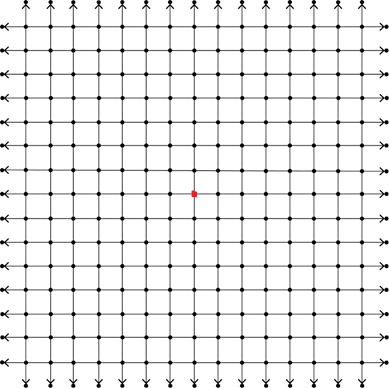
\includegraphics[scale=0.27]{game_field}
    }
    \caption{
        Рисунок 1. Скриншот приложения Random Walk Game. Строка заголовка состоит из текущего количества ходов, 
        их целей и количества ходов в самой длинной игре. Игрок видит игровое поле, положение фишки и траекторию фишки. 
        Внизу экрана показана управляющая матрица 2 на 2, которая определяет результат совместного выбора стратегий игроками A и B. 
        Строки представляют собой возможный выбор стратегий для игрока A, а столбцы – для игрока B. Результирующее направление движения 
        определяется стрелкой в ячейке, расположенной в соответствующих строке и столбце.
    }\label{fig:game_field}
\end{figure}


\subsection{Мобильное приложение и архитектура системы}\label{subsec:ch1/sec2/sub2}

Для организации экспериментальной части было разработано мобильное приложение, 
доступное в Google Play Store (https://play.google.com/store/apps/details?id=com.scigames.RWGame) и 
в AppStore (https://apps.apple.com/us/app/random-walk/id1564589250). Приложение предоставляет два режима игры: 
игра против другого игрока (PvP) или игра против среды (PvE). В обоих режимах приложение отправляет выбор игроков 
через Интернет на веб-сервер и рассчитывает направление и следующую позицию фишки на поле. Результаты игр 
(траектории и соответствующие выборы стратегий игроков на каждом ходу) были собраны в базе данных на сервере для дальнейшего анализа.

Выбор одной из двух стратегий среды в режиме PvE определяется последовательностью псевдослучайных чисел, 
вычисленных генератором случайных чисел Mersenne Twister (реализованным в PHP 7.4 как функция mt_rand) \cite{}. 
Игры, полученные в эксперименте, проводились на  поле размера 17×17.

Архитектура системы состоит из трех основных компонент: мобильное приложение, веб-сервер и база данных.
Взаимодействие между мобильным приложением и веб-сервером осуществляется посредством REST API по защищенному протоколу HTTPS
через сеть Интернет. Процесс взаимодействия клиента и сервера состоит из нескольких этапов:
\item Пользователь осуществляет регистрацию в системе, информация о регистрации отправляется на веб-сервер и сохраняется в БД.
\item Пользователь аутентифицируется в системе на основе связки логин и пароль, либо на основе OAuth аутентификации.
\item Успешная аутентификация авторизует пользователя в системе и предоставляет список текущих игр пользователя, историю игр пользователя, рейтинг участников, и возможность начать новую игру.
\item Игрок инициирует игру с другим игроком по логину, случайным образом или выбором незавершенной игры из списка.
\item После инициализации двумя игроками одной и той же игры, выбранная каждым игроком стратегия на ходе передается на веб-сервер и сохраняется в БД.
\item Клиент опрашивает веб-сервер до тех пор, пока оба игрока не совершат выбор в текущем ходе.
\item После совершения выбора обоими игроками веб-сервер определяет направление движения фишки, факт достижения границы и по запросу передает на клиент эту информацию.
\item На клиенте обновляется положение фишки, количество ходов. Игра переходит на следующий ход или завершается.

В качестве HTTP-сервера используется веб-сервер nginx \cite{}. Программная часть, реализующая функционал серверной части, 
разработана на языке PHP 7.4 \cite{} без использования дополнительных фреймворков с использованием модели Model-View-Controller \cite{}. 
Хранение информации реализовано на основе реляционной базы данных MySQL с применением хранимых процедур для защиты от XSS атак к базе данных \cite{}.
Защита паролей осуществляется с применением хеширования с солью на основе алгоритма bcrypt (реализовано в PHP 7.4 как функция password_hash).

\section{Алгоритмы и методы}\label{sec:ch1/sec3}

\subsection{Марковские цепи}\label{subsec:ch1/sec3/sub1}

\subsection{Поглощающие Марковские цепи}\label{subsec:ch1/sec3/sub2}
\subsection{Моделирование эволюции вероятности}\label{subsec:ch1/sec3/sub3}
\subsection{Численное моделирование}\label{subsec:ch1/sec3/sub4}
\subsection{Метод Монте-Карло}\label{subsec:ch1/sec3/sub5}
\subsection{Полевой эксперимент}\label{subsec:ch1/sec3/sub6}

\section{Задачи, решаемые в диссертационном исследовании}\label{sec:ch1/sec4}

\section{Выводы по главе}\label{sec:ch1/sec5}

















Мы можем сделать \textbf{жирный текст} и \textit{курсив}.

\section{Ссылки}\label{sec:ch1/sec2}

Сошлёмся на библиографию.
Одна ссылка: \cite[с.~54]{Sokolov}\cite[с.~36]{Gaidaenko}.
Две ссылки: \cite{Sokolov,Gaidaenko}.
Ссылка на собственные работы: \cite{vakbib1, confbib2}.
Много ссылок: %\cite[с.~54]{Lermontov,Management,Borozda} % такой «фокус»
%вызывает biblatex warning относительно опции sortcites, потому что неясно, к
%какому источнику относится уточнение о страницах, а bibtex об этой проблеме
%даже не предупреждает
\cite{Lermontov, Management, Borozda, Marketing, Constitution, FamilyCode,
    Gost.7.0.53, Razumovski, Lagkueva, Pokrovski, Methodology, Berestova,
    Kriger}%
\ifnumequal{\value{bibliosel}}{0}{% Примеры для bibtex8
    \cite{Sirotko, Lukina, Encyclopedia, Nasirova}%
}{% Примеры для biblatex через движок biber
    \cite{Sirotko2, Lukina2, Encyclopedia2, Nasirova2}%
}%
.
И~ещё немного ссылок:~\cite{Article,Book,Booklet,Conference,Inbook,Incollection,Manual,Mastersthesis,
    Misc,Phdthesis,Proceedings,Techreport,Unpublished}
% Следует обратить внимание, что пробел после запятой внутри \cite{}
% обрабатывается ожидаемо, а пробел перед запятой, может вызывать проблемы при
% обработке ссылок.
\cite{medvedev2006jelektronnye, CEAT:CEAT581, doi:10.1080/01932691.2010.513279,
    Gosele1999161,Li2007StressAnalysis, Shoji199895, test:eisner-sample,
    test:eisner-sample-shorted, AB_patent_Pomerantz_1968, iofis_patent1960}%
\ifnumequal{\value{bibliosel}}{0}{% Примеры для bibtex8
}{% Примеры для biblatex через движок biber
    \cite{patent2h, patent3h, patent2}%
}%
.

\ifnumequal{\value{bibliosel}}{0}{% Примеры для bibtex8
Попытка реализовать несколько ссылок на конкретные страницы
для \texttt{bibtex} реализации библиографии:
[\citenum{Sokolov}, с.~54; \citenum{Gaidaenko}, с.~36].
}{% Примеры для biblatex через движок biber
Несколько источников (мультицитата):
% Тут специально написано по-разному тире, для демонстрации, что
% применение специальных тире в настоящий момент в biblatex приводит к непоказу
% "с.".
\cites[vii--x, 5, 7]{Sokolov}[v"--~x, 25, 526]{Gaidaenko}[vii--x, 5, 7]{Techreport},
работает только в \texttt{biblatex} реализации библиографии.
}%

Ссылки на собственные работы:~\cite{vakbib1, confbib1}.

Сошлёмся на приложения: Приложение~\cref{app:A}, Приложение~\cref{app:B2}.

Сошлёмся на формулу: формула~\cref{eq:equation1}.

Сошлёмся на изображение: рисунок~\cref{fig:knuth}.

Стандартной практикой является добавление к ссылкам префикса, характеризующего тип элемента.
Это не является строгим требованием, но~позволяет лучше ориентироваться в документах большого размера.
Например, для ссылок на~рисунки используется префикс \textit{fig},
для ссылки на~таблицу "--- \textit{tab}.

В таблице \cref{tab:tab_pref} приложения~\cref{app:B4} приведён список рекомендуемых
к использованию стандартных префиксов.

В некоторых ситуациях возникает необходимость отойти от требований ГОСТ по оформлению ссылок на
литературу.
В таком случае можно воспользоваться дополнительными опциями пакета \verb+biblatex+.

Например, в ссылке на книгу~\cite{sobenin_kdv} использование опции \verb+maxnames=4+ позволяет
вывести имена всех четырёх авторов.
По ГОСТ имена последних трёх авторов опускаются.

Кроме того, часто возникают проблемы с транслитерованными инициалами. Некоторые буквы русского
алфавита по правилам транслитерации записываются двумя буквами латинского алфавита (ю-yu, ё-yo и
т.д.).
Такие инициалы \verb+biblatex+ будет сокращать до одной буквы, что неверно.
Поправить его работу можно использовав опцию \verb+giveninits=false+.
Пример использования этой опции можно видеть в ссылке~\cite{initials}.

\section{Формулы}\label{sec:ch1/sec3}

Благодаря пакету \textit{icomma}, \LaTeX~одинаково хорошо воспринимает
в~качестве десятичного разделителя и запятую (\(3,1415\)), и точку (\(3.1415\)).

\subsection{Ненумерованные одиночные формулы}\label{subsec:ch1/sec3/sub1}

Вот так может выглядеть формула, которую необходимо вставить в~строку
по~тексту: \(x \approx \sin x\) при \(x \to 0\).

А вот так выглядит ненумерованная отдельностоящая формула c подстрочными
и надстрочными индексами:
\[
    (x_1+x_2)^2 = x_1^2 + 2 x_1 x_2 + x_2^2
\]

Формула с неопределенным интегралом:
\[
    \int f(\alpha+x)=\sum\beta
\]

При использовании дробей формулы могут получаться очень высокие:
\[
    \frac{1}{\sqrt{2}+
        \displaystyle\frac{1}{\sqrt{2}+
            \displaystyle\frac{1}{\sqrt{2}+\cdots}}}
\]

В формулах можно использовать греческие буквы:
%Все \original... команды заранее, ради этого примера, определены в Dissertation\userstyles.tex
\[
    \alpha\beta\gamma\delta\originalepsilon\epsilon\zeta\eta\theta%
    \vartheta\iota\kappa\varkappa\lambda\mu\nu\xi\pi\varpi\rho\varrho%
    \sigma\varsigma\tau\upsilon\originalphi\phi\chi\psi\omega\Gamma\Delta%
    \Theta\Lambda\Xi\Pi\Sigma\Upsilon\Phi\Psi\Omega
\]
\[%https://texfaq.org/FAQ-boldgreek
    \boldsymbol{\alpha\beta\gamma\delta\originalepsilon\epsilon\zeta\eta%
        \theta\vartheta\iota\kappa\varkappa\lambda\mu\nu\xi\pi\varpi\rho%
        \varrho\sigma\varsigma\tau\upsilon\originalphi\phi\chi\psi\omega\Gamma%
        \Delta\Theta\Lambda\Xi\Pi\Sigma\Upsilon\Phi\Psi\Omega}
\]

Для добавления формул можно использовать пары \verb+$+\dots\verb+$+ и \verb+$$+\dots\verb+$$+,
но~они считаются устаревшими.
Лучше использовать их функциональные аналоги \verb+\(+\dots\verb+\)+ и \verb+\[+\dots\verb+\]+.

\subsection{Ненумерованные многострочные формулы}\label{subsec:ch1/sec3/sub2}

Вот так можно написать две формулы, не нумеруя их, чтобы знаки <<равно>> были
строго друг под другом:
\begin{align}
    f_W & =  \min \left( 1, \max \left( 0, \frac{W_{soil} / W_{max}}{W_{crit}} \right)  \right), \nonumber \\
    f_T & =  \min \left( 1, \max \left( 0, \frac{T_s / T_{melt}}{T_{crit}} \right)  \right), \nonumber
\end{align}

Выровнять систему ещё и по переменной \( x \) можно, используя окружение
\verb|alignedat| из пакета \verb|amsmath|. Вот так:
\[
|x| = \left\{
\begin{alignedat}{2}
    &&x, \quad &\text{eсли } x\geqslant 0 \\
    &-&x, \quad & \text{eсли } x<0
\end{alignedat}
\right.
\]
Здесь первый амперсанд (в исходном \LaTeX\ описании формулы) означает
выравнивание по~левому краю, второй "--- по~\( x \), а~третий "--- по~слову
<<если>>. Команда \verb|\quad| делает большой горизонтальный пробел.

Ещё вариант:
\[
    |x|=
    \begin{cases}
        \phantom{-}x, \text{если } x \geqslant 0 \\
        -x, \text{если } x<0
    \end{cases}
\]

Кроме того, для  нумерованных формул \verb|alignedat| делает вертикальное
выравнивание номера формулы по центру формулы. Например, выравнивание
компонент вектора:
\begin{equation}
    \label{eq:2p3}
    \begin{alignedat}{2}
        {\mathbf{N}}_{o1n}^{(j)} = \,{\sin} \phi\,n\!\left(n+1\right)
        {\sin}\theta\,
        \pi_n\!\left({\cos} \theta\right)
        \frac{
        z_n^{(j)}\!\left( \rho \right)
        }{\rho}\,
        &{\boldsymbol{\hat{\mathrm e}}}_{r}\,+   \\
        +\,
        {\sin} \phi\,
        \tau_n\!\left({\cos} \theta\right)
        \frac{
        \left[\rho z_n^{(j)}\!\left( \rho \right)\right]^{\prime}
        }{\rho}\,
        &{\boldsymbol{\hat{\mathrm e}}}_{\theta}\,+   \\
        +\,
        {\cos} \phi\,
        \pi_n\!\left({\cos} \theta\right)
        \frac{
        \left[\rho z_n^{(j)}\!\left( \rho \right)\right]^{\prime}
        }{\rho}\,
        &{\boldsymbol{\hat{\mathrm e}}}_{\phi}\:.
    \end{alignedat}
\end{equation}

Ещё об отступах. Иногда для лучшей <<читаемости>> формул полезно
немного исправить стандартные интервалы \LaTeX\ с учётом логической
структуры самой формулы. Например в формуле~\cref{eq:2p3} добавлен
небольшой отступ \verb+\,+ между основными сомножителями, ниже
результат применения всех вариантов отступа:
\begin{align*}
    \backslash!             & \quad f(x) = x^2\! +3x\! +2         \\
    \mbox{по-умолчанию}     & \quad f(x) = x^2+3x+2               \\
    \backslash,             & \quad f(x) = x^2\, +3x\, +2         \\
    \backslash{:}           & \quad f(x) = x^2\: +3x\: +2         \\
    \backslash;             & \quad f(x) = x^2\; +3x\; +2         \\
    \backslash \mbox{space} & \quad f(x) = x^2\ +3x\ +2           \\
    \backslash \mbox{quad}  & \quad f(x) = x^2\quad +3x\quad +2   \\
    \backslash \mbox{qquad} & \quad f(x) = x^2\qquad +3x\qquad +2
\end{align*}

Можно использовать разные математические алфавиты:
\begin{align}
    \mathcal{ABCDEFGHIJKLMNOPQRSTUVWXYZ} \nonumber  \\
    \mathfrak{ABCDEFGHIJKLMNOPQRSTUVWXYZ} \nonumber \\
    \mathbb{ABCDEFGHIJKLMNOPQRSTUVWXYZ} \nonumber
\end{align}

Посмотрим на систему уравнений на примере аттрактора Лоренца:

\[
\left\{
\begin{array}{rl}
    \dot x = & \sigma (y-x)  \\
    \dot y = & x (r - z) - y \\
    \dot z = & xy - bz
\end{array}
\right.
\]

А для вёрстки матриц удобно использовать многоточия:
\[
    \left(
        \begin{array}{ccc}
            a_{11} & \ldots & a_{1n} \\
            \vdots & \ddots & \vdots \\
            a_{n1} & \ldots & a_{nn} \\
        \end{array}
    \right)
\]

\subsection{Нумерованные формулы}\label{subsec:ch1/sec3/sub3}

А вот так пишется нумерованная формула:
\begin{equation}
    \label{eq:equation1}
    e = \lim_{n \to \infty} \left( 1+\frac{1}{n} \right) ^n
\end{equation}

Нумерованных формул может быть несколько:
\begin{equation}
    \label{eq:equation2}
    \lim_{n \to \infty} \sum_{k=1}^n \frac{1}{k^2} = \frac{\pi^2}{6}
\end{equation}

Впоследствии на формулы~\cref{eq:equation1, eq:equation2} можно ссылаться.

Сделать так, чтобы номер формулы стоял напротив средней строки, можно,
используя окружение \verb|multlined| (пакет \verb|mathtools|) вместо
\verb|multline| внутри окружения \verb|equation|. Вот так:
\begin{equation} % \tag{S} % tag - вписывает свой текст
    \label{eq:equation3}
    \begin{multlined}
        1+ 2+3+4+5+6+7+\dots + \\
        + 50+51+52+53+54+55+56+57 + \dots + \\
        + 96+97+98+99+100=5050
    \end{multlined}
\end{equation}

Уравнения~\cref{eq:subeq_1,eq:subeq_2} демонстрируют возможности
окружения \verb|\subequations|.
\begin{subequations}
    \label{eq:subeq_1}
    \begin{gather}
        y = x^2 + 1 \label{eq:subeq_1-1} \\
        y = 2 x^2 - x + 1 \label{eq:subeq_1-2}
    \end{gather}
\end{subequations}
Ссылки на отдельные уравнения~\cref{eq:subeq_1-1,eq:subeq_1-2,eq:subeq_2-1}.
\begin{subequations}
    \label{eq:subeq_2}
    \begin{align}
        y & = x^3 + x^2 + x + 1 \label{eq:subeq_2-1} \\
        y & = x^2
    \end{align}
\end{subequations}

\subsection{Форматирование чисел и размерностей величин}\label{sec:units}

Числа форматируются при помощи команды \verb|\num|:
\num{5,3};
\num{2,3e8};
\num{12345,67890};
\num{2,6 d4};
\num{1+-2i};
\num{.3e45};
\num[exponent-base=2]{5 e64};
\num[exponent-base=2,exponent-to-prefix]{5 e64};
\num{1.654 x 2.34 x 3.430}
\num{1 2 x 3 / 4}.
Для написания последовательности чисел можно использовать команды \verb|\numlist| и \verb|\numrange|:
\numlist{10;30;50;70}; \numrange{10}{30}.
Значения углов можно форматировать при помощи команды \verb|\ang|:
\ang{2.67};
\ang{30,3};
\ang{-1;;};
\ang{;-2;};
\ang{;;-3};
\ang{300;10;1}.

Обратите внимание, что ГОСТ запрещает использование знака <<->> для обозначения отрицательных чисел
за исключением формул, таблиц и~рисунков.
Вместо него следует использовать слово <<минус>>.

Размерности можно записывать при помощи команд \verb|\si| и \verb|\SI|:
\si{\farad\squared\lumen\candela};
\si{\joule\per\mole\per\kelvin};
\si[per-mode = symbol-or-fraction]{\joule\per\mole\per\kelvin};
\si{\metre\per\second\squared};
\SI{0.10(5)}{\neper};
\SI{1.2-3i e5}{\joule\per\mole\per\kelvin};
\SIlist{1;2;3;4}{\tesla};
\SIrange{50}{100}{\volt}.
Список единиц измерений приведён в таблицах~\cref{tab:unit:base,
    tab:unit:derived,tab:unit:accepted,tab:unit:physical,tab:unit:other}.
Приставки единиц приведены в~таблице~\cref{tab:unit:prefix}.

С дополнительными опциями форматирования можно ознакомиться в~описании пакета \texttt{siunitx};
изменить или добавить единицы измерений можно в~файле \texttt{siunitx.cfg}.

\begin{table}
    \centering
    \captionsetup{justification=centering} % выравнивание подписи по-центру
    \caption{Основные величины СИ}\label{tab:unit:base}
    \begin{tabular}{llc}
        \toprule
        Название  & Команда                 & Символ         \\
        \midrule
        Ампер     & \verb|\ampere| & \si{\ampere}   \\
        Кандела   & \verb|\candela| & \si{\candela}  \\
        Кельвин   & \verb|\kelvin| & \si{\kelvin}   \\
        Килограмм & \verb|\kilogram| & \si{\kilogram} \\
        Метр      & \verb|\metre| & \si{\metre}    \\
        Моль      & \verb|\mole| & \si{\mole}     \\
        Секунда   & \verb|\second| & \si{\second}   \\
        \bottomrule
    \end{tabular}
\end{table}

\begin{table}
    \small
    \centering
    \begin{threeparttable}% выравнивание подписи по границам таблицы
        \caption{Производные единицы СИ}\label{tab:unit:derived}
        \begin{tabular}{llc|llc}
            \toprule
            Название       & Команда                 & Символ              & Название & Команда & Символ \\
            \midrule
            Беккерель      & \verb|\becquerel| & \si{\becquerel}     &
            Ньютон         & \verb|\newton| & \si{\newton}                                      \\
            Градус Цельсия & \verb|\degreeCelsius| & \si{\degreeCelsius} &
            Ом             & \verb|\ohm| & \si{\ohm}                                         \\
            Кулон          & \verb|\coulomb| & \si{\coulomb}       &
            Паскаль        & \verb|\pascal| & \si{\pascal}                                      \\
            Фарад          & \verb|\farad| & \si{\farad}         &
            Радиан         & \verb|\radian| & \si{\radian}                                      \\
            Грей           & \verb|\gray| & \si{\gray}          &
            Сименс         & \verb|\siemens| & \si{\siemens}                                     \\
            Герц           & \verb|\hertz| & \si{\hertz}         &
            Зиверт         & \verb|\sievert| & \si{\sievert}                                     \\
            Генри          & \verb|\henry| & \si{\henry}         &
            Стерадиан      & \verb|\steradian| & \si{\steradian}                                   \\
            Джоуль         & \verb|\joule| & \si{\joule}         &
            Тесла          & \verb|\tesla| & \si{\tesla}                                       \\
            Катал          & \verb|\katal| & \si{\katal}         &
            Вольт          & \verb|\volt| & \si{\volt}                                        \\
            Люмен          & \verb|\lumen| & \si{\lumen}         &
            Ватт           & \verb|\watt| & \si{\watt}                                        \\
            Люкс           & \verb|\lux| & \si{\lux}           &
            Вебер          & \verb|\weber| & \si{\weber}                                       \\
            \bottomrule
        \end{tabular}
    \end{threeparttable}
\end{table}

\begin{table}
    \centering
    \begin{threeparttable}% выравнивание подписи по границам таблицы
        \caption{Внесистемные единицы}\label{tab:unit:accepted}

        \begin{tabular}{llc}
            \toprule
            Название        & Команда                 & Символ          \\
            \midrule
            День            & \verb|\day| & \si{\day}       \\
            Градус          & \verb|\degree| & \si{\degree}    \\
            Гектар          & \verb|\hectare| & \si{\hectare}   \\
            Час             & \verb|\hour| & \si{\hour}      \\
            Литр            & \verb|\litre| & \si{\litre}     \\
            Угловая минута  & \verb|\arcminute| & \si{\arcminute} \\
            Угловая секунда & \verb|\arcsecond| & \si{\arcsecond} \\ %
            Минута          & \verb|\minute| & \si{\minute}    \\
            Тонна           & \verb|\tonne| & \si{\tonne}     \\
            \bottomrule
        \end{tabular}
    \end{threeparttable}
\end{table}

\begin{table}
    \centering
    \captionsetup{justification=centering}
    \caption{Внесистемные единицы, получаемые из эксперимента}\label{tab:unit:physical}
    \begin{tabular}{llc}
        \toprule
        Название                & Команда                 & Символ                 \\
        \midrule
        Астрономическая единица & \verb|\astronomicalunit| & \si{\astronomicalunit} \\
        Атомная единица массы   & \verb|\atomicmassunit| & \si{\atomicmassunit}   \\
        Боровский радиус        & \verb|\bohr| & \si{\bohr}             \\
        Скорость света          & \verb|\clight| & \si{\clight}           \\
        Дальтон                 & \verb|\dalton| & \si{\dalton}           \\
        Масса электрона         & \verb|\electronmass| & \si{\electronmass}     \\
        Электрон Вольт          & \verb|\electronvolt| & \si{\electronvolt}     \\
        Элементарный заряд      & \verb|\elementarycharge| & \si{\elementarycharge} \\
        Энергия Хартри          & \verb|\hartree| & \si{\hartree}          \\
        Постоянная Планка       & \verb|\planckbar| & \si{\planckbar}        \\
        \bottomrule
    \end{tabular}
\end{table}

\begin{table}
    \centering
    \begin{threeparttable}% выравнивание подписи по границам таблицы
        \caption{Другие внесистемные единицы}\label{tab:unit:other}
        \begin{tabular}{llc}
            \toprule
            Название                  & Команда                 & Символ             \\
            \midrule
            Ангстрем                  & \verb|\angstrom| & \si{\angstrom}     \\
            Бар                       & \verb|\bar| & \si{\bar}          \\
            Барн                      & \verb|\barn| & \si{\barn}         \\
            Бел                       & \verb|\bel| & \si{\bel}          \\
            Децибел                   & \verb|\decibel| & \si{\decibel}      \\
            Узел                      & \verb|\knot| & \si{\knot}         \\
            Миллиметр ртутного столба & \verb|\mmHg| & \si{\mmHg}         \\
            Морская миля              & \verb|\nauticalmile| & \si{\nauticalmile} \\
            Непер                     & \verb|\neper| & \si{\neper}        \\
            \bottomrule
        \end{tabular}
    \end{threeparttable}
\end{table}

\begin{table}
    \small
    \centering
    \begin{threeparttable}% выравнивание подписи по границам таблицы
        \caption{Приставки СИ}\label{tab:unit:prefix}
        \begin{tabular}{llcc|llcc}
            \toprule
            Приставка & Команда                  & Символ      & Степень &
            Приставка & Команда                  & Символ      & Степень   \\
            \midrule
            Иокто     & \verb|\yocto|  & \si{\yocto} & -24     &
            Дека      & \verb|\deca|  & \si{\deca}  & 1         \\
            Зепто     & \verb|\zepto|  & \si{\zepto} & -21     &
            Гекто     & \verb|\hecto|  & \si{\hecto} & 2         \\
            Атто      & \verb|\atto|  & \si{\atto}  & -18     &
            Кило      & \verb|\kilo|  & \si{\kilo}  & 3         \\
            Фемто     & \verb|\femto|  & \si{\femto} & -15     &
            Мега      & \verb|\mega|  & \si{\mega}  & 6         \\
            Пико      & \verb|\pico|  & \si{\pico}  & -12     &
            Гига      & \verb|\giga|  & \si{\giga}  & 9         \\
            Нано      & \verb|\nano|  & \si{\nano}  & -9      &
            Терра     & \verb|\tera|  & \si{\tera}  & 12        \\
            Микро     & \verb|\micro|  & \si{\micro} & -6      &
            Пета      & \verb|\peta|  & \si{\peta}  & 15        \\
            Милли     & \verb|\milli|  & \si{\milli} & -3      &
            Екса      & \verb|\exa|  & \si{\exa}   & 18        \\
            Санти     & \verb|\centi|  & \si{\centi} & -2      &
            Зетта     & \verb|\zetta|  & \si{\zetta} & 21        \\
            Деци      & \verb|\deci| & \si{\deci}  & -1      &
            Иотта     & \verb|\yotta| & \si{\yotta} & 24        \\
            \bottomrule
        \end{tabular}
    \end{threeparttable}
\end{table}

\subsection{Заголовки с формулами: \texorpdfstring{\(a^2 + b^2 = c^2\)}{%
        a\texttwosuperior\ + b\texttwosuperior\ = c\texttwosuperior},
    \texorpdfstring{\(\left\vert\textrm{{Im}}\Sigma\left(
            \protect\varepsilon\right)\right\vert\approx const\)}{|ImΣ (ε)| ≈ const},
    \texorpdfstring{\(\sigma_{xx}^{(1)}\)}{σ\_\{xx\}\textasciicircum\{(1)\}}
}\label{subsec:with_math}

Пакет \texttt{hyperref} берёт текст для закладок в pdf-файле из~аргументов
команд типа \verb|\section|, которые могут содержать математические формулы,
а~также изменения цвета текста или шрифта, которые не отображаются в~закладках.
Чтобы использование формул в заголовках не вызывало в~логе компиляции появление
предупреждений типа <<\texttt{Token not allowed in~a~PDF string
    (Unicode):(hyperref) removing...}>>, следует использовать конструкцию
\verb|\texorpdfstring{}{}|, где в~первых фигурных скобках указывается
формула, а~во~вторых "--- запись формулы для закладок.

\section{Рецензирование текста}\label{sec:markup}

В шаблоне для диссертации и автореферата заданы команды рецензирования.
Они видны при компиляции шаблона в режиме черновика или при установке
соответствующей настройки (\verb+showmarkup+) в~файле \verb+common/setup.tex+.

Команда \verb+\todo+ отмечает текст красным цветом.
\todo{Например, так.}

Команда \verb+\note+ позволяет выбрать цвет текста.
\note{Чёрный, } \note[red]{красный, } \note[green]{зелёный, }
\note[blue]{синий.} \note[orange]{Обратите внимание на ширину и расстановку
    формирующихся пробелов, в~результате приведённой записи (зависит также
    от~применяемого компилятора).}

Окружение \verb+commentbox+ также позволяет выбрать цвет.

\begin{commentbox}[red]
    Красный текст.

    Несколько параграфов красного текста.
\end{commentbox}

\begin{commentbox}[blue]
    Синяя формула.

    \begin{equation}
        \alpha + \beta = \gamma
    \end{equation}
\end{commentbox}

\verb+commentbox+ позволяет закомментировать участок кода в~режиме чистовика.
Чтобы убрать кусок кода для всех режимов, можно использовать окружение
\verb+comment+.

\begin{comment}
Этот текст всегда скрыт.
\end{comment}

\section{Работа со списком сокращений и~условных обозначений}\label{sec:acronyms}

С помощью пакета \texttt{nomencl} можно создавать удобный сортированный список
сокращений и условных обозначений во время написания текста. Вызов
\verb+\nomenclature+ добавляет нужный символ или сокращение с~описанием
в~список, который затем печатается вызовом \verb+\printnomenclature+
в~соответствующем разделе.
Для того, чтобы эти операции прошли, потребуется дополнительный вызов
\verb+makeindex -s nomencl.ist -o %.nls %.nlo+ в~командной строке, где вместо
\verb+%+ следует подставить имя главного файла проекта (\verb+dissertation+
для этого шаблона).
Затем потребуется один или два дополнительных вызова компилятора проекта.
\begin{equation}
    \omega = c k,
\end{equation}
где \( \omega \) "--- частота света, \( c \) "--- скорость света, \( k \) "---
модуль волнового вектора.
\nomenclature{\(\omega\)}{частота света\nomrefeq}
\nomenclature{\(c\)}{скорость света\nomrefpage}
\nomenclature{\(k\)}{модуль волнового вектора\nomrefeqpage}
Использование
\begin{verbatim}
\nomenclature{\(\omega\)}{частота света\nomrefeq}
\nomenclature{\(c\)}{скорость света\nomrefpage}
\nomenclature{\(k\)}{модуль волнового вектора\nomrefeqpage}
\end{verbatim}
после уравнения добавит в список условных обозначений три записи.
Ссылки \verb+\nomrefeq+ на последнее уравнение, \verb+\nomrefpage+ "--- на
страницу, \verb+\nomrefeqpage+ "--- сразу на~последнее уравнение и~на~страницу,
можно опускать и~не~использовать.

Группировкой и сортировкой пунктов в списке можно управлять с~помощью указания
дополнительных аргументов к команде \verb+nomenclature+.
Например, при вызове
\begin{verbatim}
\nomenclature[03]{\( \hbar \)}{постоянная Планка}
\nomenclature[01]{\( G \)}{гравитационная постоянная}
\end{verbatim}
\( G \) будет стоять в списке выше, чем \( \hbar \).
Для корректных вертикальных отступов между строками в описании лучше
не~использовать многострочные формулы в~списке обозначений.

\nomenclature{%
    \( \begin{rcases}
        a_n \\
        b_n
    \end{rcases} \)%
}{коэффициенты разложения Ми в дальнем поле соответствующие электрическим и
    магнитным мультиполям}
\nomenclature[a\( e \)]{\( {\boldsymbol{\hat{\mathrm e}}} \)}{единичный вектор}
\nomenclature{\( E_0 \)}{амплитуда падающего поля}
\nomenclature{\( j \)}{тип функции Бесселя}
\nomenclature{\( k \)}{волновой вектор падающей волны}
\nomenclature{%
    \( \begin{rcases}
        a_n \\
        b_n
    \end{rcases} \)%
}{и снова коэффициенты разложения Ми в дальнем поле соответствующие
    электрическим и магнитным мультиполям. Добавлено много текста, так что
    описание группы условных обозначений значительно превысило высоту этой
    группы...}
\nomenclature{\( L \)}{общее число слоёв}
\nomenclature{\( l \)}{номер слоя внутри стратифицированной сферы}
\nomenclature{\( \lambda \)}{длина волны электромагнитного излучения в вакууме}
\nomenclature{\( n \)}{порядок мультиполя}
\nomenclature{%
    \( \begin{rcases}
        {\mathbf{N}}_{e1n}^{(j)} & {\mathbf{N}}_{o1n}^{(j)} \\
        {\mathbf{M}_{o1n}^{(j)}} & {\mathbf{M}_{e1n}^{(j)}}
    \end{rcases} \)%
}{сферические векторные гармоники}
\nomenclature{\( \mu \)}{магнитная проницаемость в вакууме}
\nomenclature{\( r, \theta, \phi \)}{полярные координаты}
\nomenclature{\( \omega \)}{частота падающей волны}

С помощью \verb+nomenclature+ можно включать в~список сокращения,
не~используя их~в~тексте.
% запись сокращения в список происходит командой \nomenclature,
% а не употреблением самого сокращения
\nomenclature{FEM}{finite element method, метод конечных элементов}
\nomenclature{FIT}{finite integration technique, метод конечных интегралов}
\nomenclature{FMM}{fast multipole method, быстрый метод многополюсника}
\nomenclature{FVTD}{finite volume time-domain, метод конечных объёмов
    во~временной области}
\nomenclature{MLFMA}{multilevel fast multipole algorithm, многоуровневый
    быстрый алгоритм многополюсника}
\nomenclature{BEM}{boundary element method, метод граничных элементов}
\nomenclature{CST MWS}{Computer Simulation Technology Microwave Studio
    программа для компьютерного моделирования уравнен Максвелла}
\nomenclature{DDA}{discrete dipole approximation, приближение дискретиных
    диполей}
\nomenclature{FDFD}{finite difference frequency domain, метод конечных
    разностей в~частотной области}
\nomenclature{FDTD}{finite difference time domain, метод конечных разностей
    во~временной области}
\nomenclature{MoM}{method of moments, метод моментов}
\nomenclature{MSTM}{multiple sphere T-Matrix, метод Т-матриц для множества
    сфер}
\nomenclature{PSTD}{pseudospectral time domain method, псевдоспектральный метод
    во~временной области}
\nomenclature{TLM}{transmission line matrix method, метод матриц линий передач}

\FloatBarrier
